\documentclass[a4paper,12pt]{article}

\title{Biology 30 IB \\ Nervous System}
\author{Jad Chehimi}

% document setup
\renewcommand{\familydefault}{\sfdefault}
\linespread{1.25}
\usepackage[margin=1in]{geometry}
\usepackage{setspace}
\usepackage{enumitem}
\setlist{nosep}
\usepackage{color,soul}
\setcounter{secnumdepth}{0}

% tools
\usepackage[hidelinks]{hyperref}
\usepackage{float}
%% images
\usepackage{graphicx}
\graphicspath{ {./images/} }
%% science
\usepackage{siunitx}
%% chemistry
\usepackage[version=4]{mhchem}

\begin{document}
\maketitle

\tableofcontents

\pagebreak

\section{(13.1) The Nervous System}
\begin{itemize}
    \item{\textbf{Equilibrium/Homeostasis} = balance, main job of nervous system is to maintain this}
    \item{
            Nervous system contains...
            \begin{itemize}
                \item{Brain}
                \item{Spinal cord}
                \item{Nerves}
            \end{itemize}
        }
\end{itemize}

\section{Divisions of the Nervous System}
\begin{figure}[H]
    \centering
    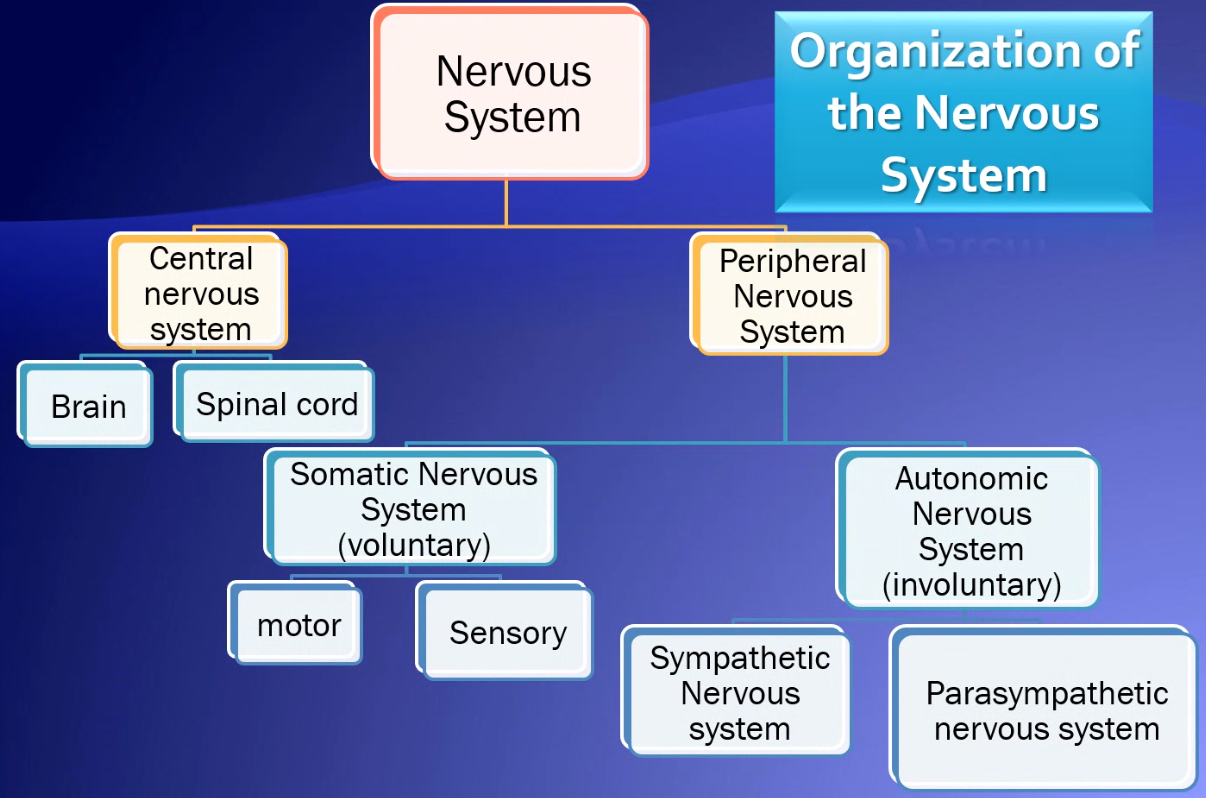
\includegraphics[width=\textwidth]{flowchart}
\end{figure}

\subsection{Central Nervous System (CNS)}
\begin{itemize}
    \item{Integrates and processes information}
    \item{Consists of \hl{brain} and \hl{spinal cord}}
\end{itemize}

\subsection{Peripheral Nervous System (PNS)}
\begin{itemize}
    \item{\hl{Messenger nerves}; bring \hl{info to and from} the central nervous system}
    \item{
            Each include two types of neurons...
            \begin{itemize}
                \item{\textbf{Sensory receptors} = carry sensory info to the CNS}
                \item{\textbf{Motor neurons} = \hl{voluntary motor/muscle control}, carry signals from the CNS to the skeletal muscles}
            \end{itemize}
        }

\end{itemize}

\subsubsection{Somatic Nervous System (SNS)}
\begin{itemize}
    \item{Voluntary control}
    \item{\hl{Somatic sensory neurons} gather info from external stimuli --- \hl{five senses}}
    \item{\hl{Somatic motor neurons} control voluntary skeletal muscles}
\end{itemize}

\subsubsection{Autonomic Nervous System (ANS)}
\begin{itemize}
    \item{Divisions of automatic nerves that are \hl{antagonistic/oppose each other}}
    \item{Regulates involuntary control processes (automatic), such as breathing and heartbeat}
    \item{\hl{Autonomic sensory neurons} gather info from internal stimuli --- involved with blood pressure and heart rate}
    \item{Autonomic motor neurons control glandular secretions and the function of \hl{smooth and cardiac muscles}}
\end{itemize}

\textbf{Sympathetic Nervous System}
\begin{itemize}
    \item{"Fight or flight (or freeze)" responses}
    \item{\hl{Prioritizes urgent} functions, such as by speeding up rates of breathing, heart rate, etc.}
    \item{\hl{Disables non-urgent} functions, such as digesting}
\end{itemize}

\textbf{Parasympathetic Nervous System}
\begin{itemize}
    \item{"Rest and digest" responses}
    \item{\hl{Restores normal priorities}, slows down rates of breathing, heart rate, etc.}
    \item{\hl{Re-enables non-urgent} functions, such as digesting}
\end{itemize}

\pagebreak

\section{Cells of the Nervous System}
\subsection{Neurons}
Functional units of nervous system, \hl{tissues of neurons} are called \textbf{nerves}.
\begin{itemize}
    \item{\hl{Respond} to physical and chemical stimuli}
    \item{\hl{Conduct} electrochemical signals}
    \item{\hl{Release} chemicals that regulate various body processes}
\end{itemize}

\subsubsection{Types of Neurons}
\begin{itemize}
    \item{\textbf{Sensory receptors} = recieves info from 5 senses; bulb-like, end part of sensory neuron}
    \item{\textbf{Sensory neurons} = gather \hl{info from sensory} receptors, transmits \hl{to CNS}}
    \item{\textbf{Interneurons} = only in CNS; link \hl{between sensory and motor} neurons}
    \item{\textbf{Motor neurons} = transmit info from \hl{CNS to effectors}}
    \item{\textbf{Effectors} = muscles, glands, other organs}
\end{itemize}

\subsection{Glial Cells}
Supporting cells of nerve cells.
\begin{itemize}
    \item{Nourish neurons, remove wastes, \& defend against infection}
    \item{Provide a supporting framework for all nervous-system tissue}
\end{itemize}

\pagebreak

\section{Neuron Anatomy}

\begin{figure}[H]
    \centering
    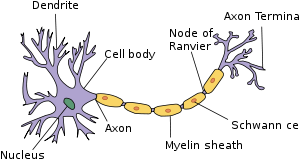
\includegraphics[width=\textwidth]{neuron}
\end{figure}

\subsection{Dendrites}
\begin{itemize}
    \item{Short, branching terminals of neuron}
    \item{
            Recieves info from...
            \begin{itemize}
                \item{other neurons}
                \item{senses (making it a \textbf{sensory receptor})}
            \end{itemize}
        }
    \item{Sends info to cell body}
\end{itemize}

\subsection{Cell Body}
\begin{itemize}
    \item{Site of metabolic reactions}
    \item{Contains a nucleus to process info from dendrites}
    \item{Makes a decision}
\end{itemize}

\subsection{Axon}
\begin{itemize}
    \item{Thread-like component of neuron after cell body}
    \item{Conducts impulses away from the cell body}
    \item{\hl{Axon terminals} = axon ends branch into many fibres}
\end{itemize}

\subsection{Myelin Sheath}
\begin{figure}[H]
    \centering
    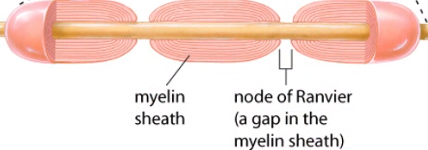
\includegraphics[width=0.50\textwidth]{ranvier}
\end{figure}

\begin{itemize}
    \item{Insulation on neurons; \hl{not all neurons} have myelin sheath}
    \item{\hl{Prevents loss} of charged \hl{ions}}
\end{itemize}

\subsubsection{Schwann Cells}
\begin{itemize}
    \item{\textbf{Schwann Cells} = glial cells \hl{wrapping around axon}; wrapped form = myelin sheath}
    \item{\textbf{White matter} = \hl{myelinated/insulated} neurons; slower than grey}
    \item{\textbf{Grey matter} = \hl{unmyelinated/exposed} neurons; common on brain surface}
    \item{
            \textbf{Neurilemma}
            \begin{itemize}
                \item{promotes the \hl{regeneration of damaged axons}}
                \item{some, \hl{not all}, schwann cells form this additional layer \hl{over the myelin sheath}}
                \item{not present in unmyelianted, grey matter (common in CNS)}
            \end{itemize}
        }

\end{itemize}

\subsubsection{Node of Ranvier}
\begin{itemize}
    \item{\hl{Gap} between myelin sheaths}
    \item{Nerve impulses \hl{"jump" from node to node}, speeding up movement}
\end{itemize}

\section{Repairing Damage Nerves}
\subsection{Stem Cells}
\begin{itemize}
    \item{Unspecialized cells}
    \item{Can be used to repair all sorts of injuries}
\end{itemize}

\subsection{Reflex Arc}
\begin{itemize}
    \item{\hl{Prevents injury} before even being consciously aware of a threat}
    \item{\textbf{Reflexes} = sudden, unlearned, and involuntary responses to certain stimuli}
    \item{
            \textbf{Spinal Reflex}
            \begin{itemize}
                \item{Reflex with no brain involvement during threat}
                \item{Decision to reflex made by interneuron}
                \item{Interneuron communicates to brain after threat}
                \item{Occurs for spinal reflexes AND conditional reflexes (e.g. touching something hot)}
                \item{Stimulus \\ $\longrightarrow$ Sensory Receptor (dendrite) $\longrightarrow$ Sensory Neuron $\longrightarrow$ Interneuron (in spine) $\longrightarrow$ Motor Neuron $\longrightarrow$ Effector Organ $\longrightarrow$ Response}
            \end{itemize}
        }
    \item{
        Severing the motor neurons in a reflex arc would cause...
        \begin{itemize}
            \item{\hl{Inability to move} the part}
            \item{\hl{Ability to feel}}
        \end{itemize}
    }
\end{itemize}

\section{(13.2) Electrochemical Impulses}
\begin{itemize}
    \item{\textbf{Intracellular fluid (ICF)} = fluid within axon}
    \item{\textbf{Extracellular fluid (ECF)} = fluid around axon}
\end{itemize}

\subsection{Resting Potential}
\begin{itemize}
    \item{Resting nerve}
    \item{Charge inside = \SI{-70}{\mV}}
    \item{Polarized (negative voltage)}
\end{itemize}

\subsection{Action Potential}
\begin{itemize}
    \item{Excited nerve}
    \item{Charge inside = +\SI{40}{\mV}}
    \item{Lasts milliseconds}
    \item{Depolarized (positive voltage)}
\end{itemize}

\subsection{Process}
\subsubsection{Summary}
\begin{itemize}
    \item{\ce{K+} leave axon = negative, polarized}
    \item{\ce{Na+} enter axon = positive, depolarized}
\end{itemize}

\pagebreak

\subsubsection{Detailed}
\begin{figure}[H]
    \centering
    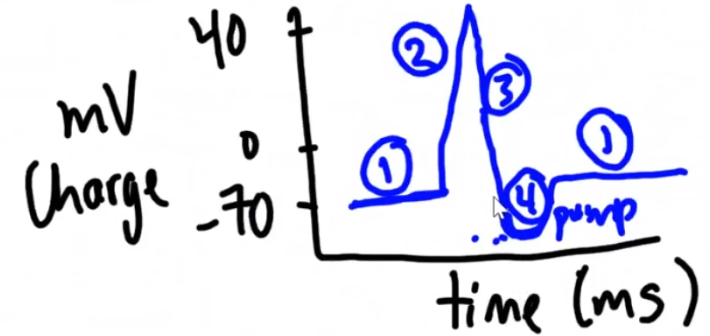
\includegraphics[width=0.7\textwidth]{ngraph}
\end{figure}
\begin{enumerate}
    \item{
            \textbf{Polarization (resting)}
            \begin{figure}[H]
                \centering
                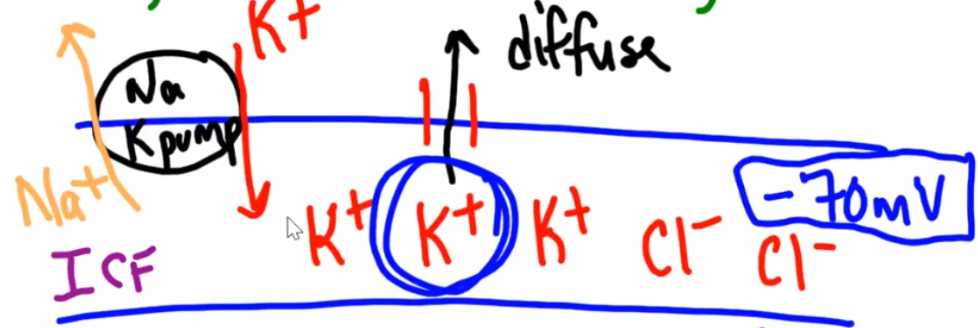
\includegraphics[width=0.7\textwidth]{n1}
            \end{figure}
            \begin{itemize}
                \item{Na/K pump pushes \ce{Na+} out of axon, and brings \ce{K+} into axon}
                \item{Some \ce{K+} passively diffuses out, charge is still negative due to \ce{Cl-} in axon}
                \item{Charge is back to \SI{-70}{\mV}}
            \end{itemize}
        }
    \item{
            \textbf{Depolarization (action potential)}
            \begin{figure}[H]
                \centering
                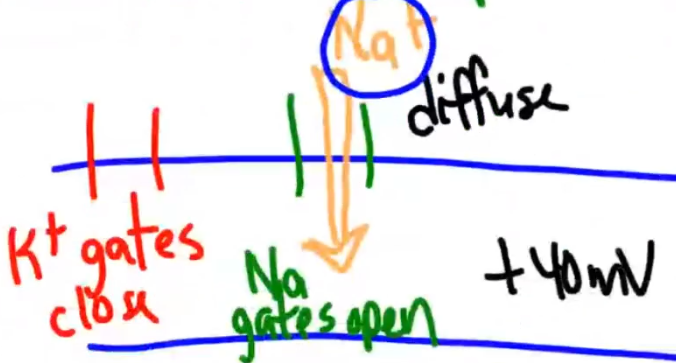
\includegraphics[width=0.7\textwidth]{n2}
            \end{figure}
            \begin{itemize}
                \item{\ce{K+} gates close}
                \item{\ce{Na+} gates open, \ce{Na+} flood in}
                \item{Charge jumps to +\SI{40}{\mV}}
            \end{itemize}
        }
    \item{
            \textbf{Repolarization}
            \begin{figure}[H]
                \centering
                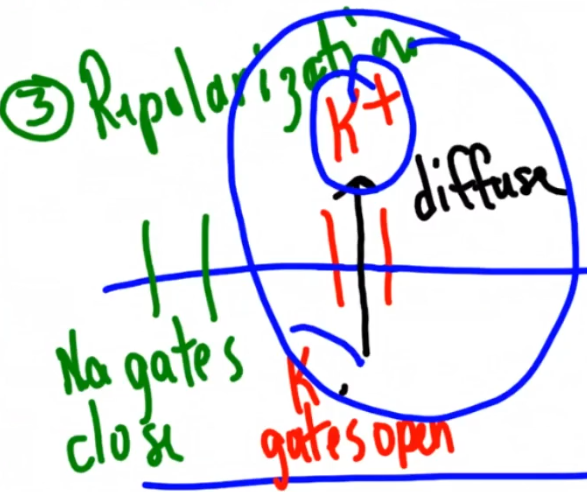
\includegraphics[width=0.60\textwidth]{n3}
            \end{figure}
            \begin{itemize}
                \item{\hl{Reestablishing a potential difference across the membrane resulting in a more negative charge inside the neuron}}
                \item{\ce{Na+} gates close}
                \item{\ce{K+} gates open}
                \item{Some \ce{K+} slowly diffuse out}
                \item{Charge lowers}
            \end{itemize}
        }
    \item{
            \textbf{Hyperpolarization}
            \begin{figure}[H]
                \centering
                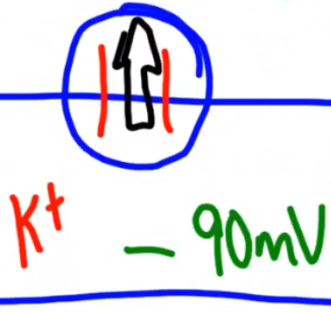
\includegraphics[width=0.40\textwidth]{n4}
            \end{figure}
            \begin{itemize}
                \item{\hl{The potential difference across the membrane is less than that of polarized neurons}}
                \item{More \ce{K+} quickly diffuse out}
                \item{Charge is now \SI{-90}{\mV}}
                \item{
                        \textbf{Recovery Period}
                        \begin{itemize}
                            \item{Negative allows neuron to rest for a few milliseconds}
                            \item{Prevents action potential from going backwards}
                        \end{itemize}
                    }
                \item{The \ce{Na+} / \ce{K+} pump is \hl{integral in this step}}
            \end{itemize}
        }
\end{enumerate}
\begin{figure}[H]
    \centering
    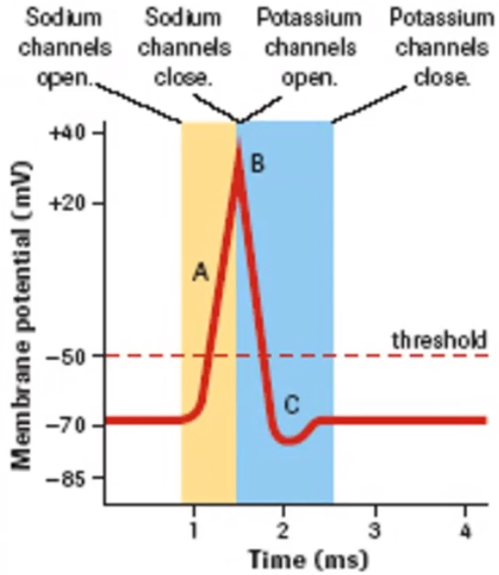
\includegraphics[width=0.40\textwidth]{ngraph2}
\end{figure}

\section{Wave of Depolarization}
\begin{itemize}
    \item{The \hl{action potential does not move}}
    \item{Rather, many action potentials are generated \hl{one after another} along the cell membrane}
    \item{Often described as like dominos}
\end{itemize}
\begin{figure}[H]
    \centering
    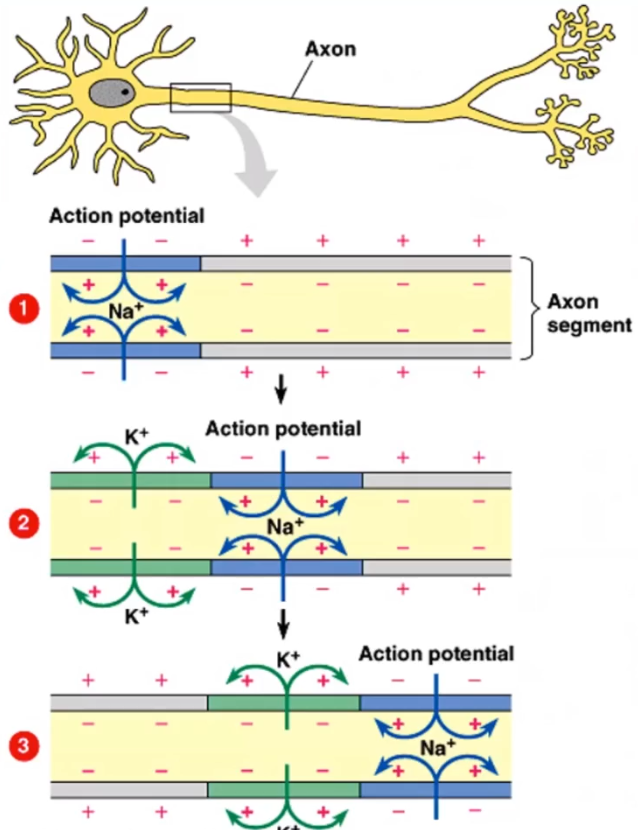
\includegraphics[width=0.60\textwidth]{wave}
\end{figure}

\section{Saltatory Conduction}
\begin{itemize}
    \item{In myelinated axons}
    \item{Action potentials "jump" from node to node between myelin sheath gaps}
    \item{Nodes of Ranvier have \hl{concentrated ion channels}}
    \item{Sodium ions (\ce{Na+}) flood the channels in the gaps, "pushing" the action potential far enough to reach the next gap}
\end{itemize}
\begin{figure}[H]
    \centering
    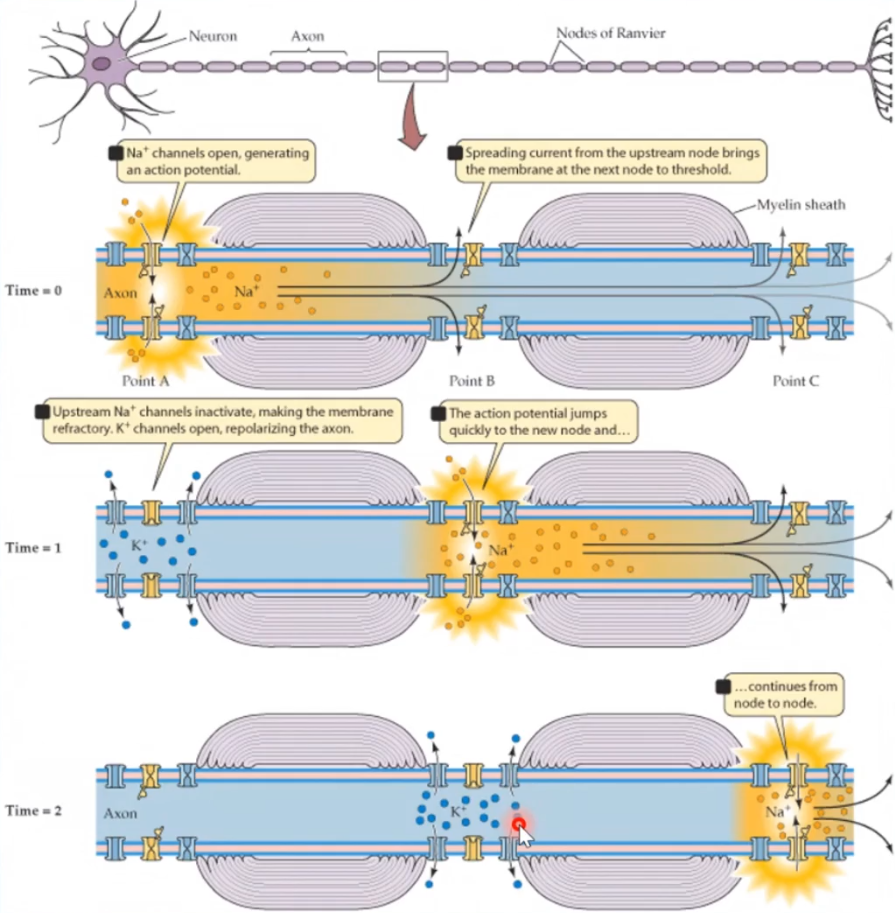
\includegraphics[width=0.9\textwidth]{salt}
\end{figure}

\subsection{This is Faster}
\begin{itemize}
    \item{Myelinated neurons utilize saltatory conduction to increase the speed of nerve impulses}
    \item{Non-myelinated neurons cannot do this, and invertebrates --- such as \hl{earthworms and squid} --- only have non-myelinated}
    \item{They evolved to have \hl{thicker axon diameters} to speed up conduction}
\end{itemize}

\section{Threshold Levels}
\begin{itemize}
    \item{Stimuli must be \hl{above a critical value} in order to produce a response}
    \item{Threshold levels are different for each neuron}
\end{itemize}

\begin{figure}[H]
    \centering
    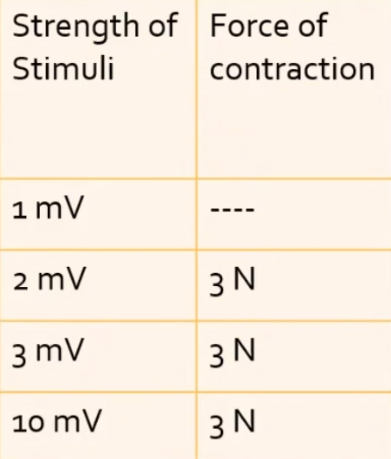
\includegraphics[width=0.3\textwidth]{threshold}
    \caption{In this example, the neuron's critical value is \SI{2}{\mV}}
\end{figure}

\subsection{All-or-none Response}
\begin{itemize}
    \item{Neurons either \hl{fire maximally or not at all}}
    \item{Stimuli intensity \hl{below} said theshold \hl{do not initiate} a response}
    \item{Stimuli intensity \hl{above} critical threshold \hl{does not produce an increased response}}
\end{itemize}

\subsection{Message Priority}
\begin{itemize}
    \item{
            An increase response is due to either...
            \begin{itemize}
                \item{\hl{more neurons} being stimulated}
                \item{some specific neurons only fire at \hl{high threshold levels}}
            \end{itemize}
        }
\end{itemize}

\begin{figure}[H]
    \centering
    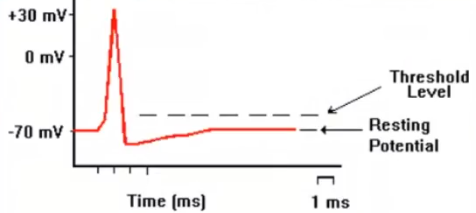
\includegraphics[width=0.6\textwidth]{threshold2}
    \caption{\ce{K+} are gradually pumped in until the threshold, then \ce{Na+} are flooded in to depolarize}
\end{figure}

\section{Neuron-to-neuron Communication}
\begin{figure}[H]
    \centering
    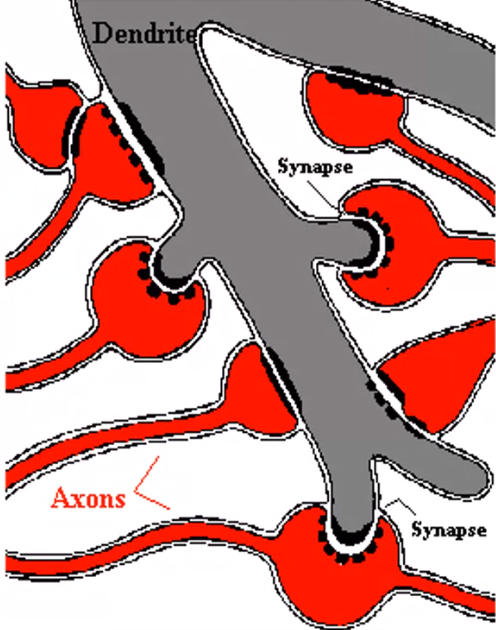
\includegraphics[width=0.5\textwidth]{synapse}
\end{figure}
\subsection{Synapse}
\begin{itemize}
    \item{\hl{Space in between two (or usually more) neurons}}
    \item{Typically around \SI{20}{\nm}}
    \item{\textbf{Presynpatic Neurons} = carry impulses to the synapse}
    \item{\textbf{Postsynaptic Neurons} = carry impulses away from synapse}
    \item{\hl{More synapses = slower transmission} (reflex arc has little synapses)}
\end{itemize}

\subsection{Neurotransmitters}
\begin{itemize}
    \item{Action potential will not move across the synapse}
    \item{\textbf{Neurotransmitters} = \hl{chemicals transported (via diffusion) between neurons across synapse}}
    \item{Always released by presynaptic neurons}
    \item{Always recieved by postsynaptic neurons}
\end{itemize}

\subsubsection{Types}
\begin{itemize}
    \item{\textbf{Excitatory} = binds to and triggers \ce{Na+} channels to open \ce{Na+} flood \hl{into postsynaptic neuron}, causing \hl{depolarization} (\ce{Na+} in)}
    \item{\textbf{Inhibitory} = binds to and triggers \ce{K+} channels to open; \hl{hyperpolarization} (\ce{K+} out)}
\end{itemize}

\begin{figure}[H]
    \centering
    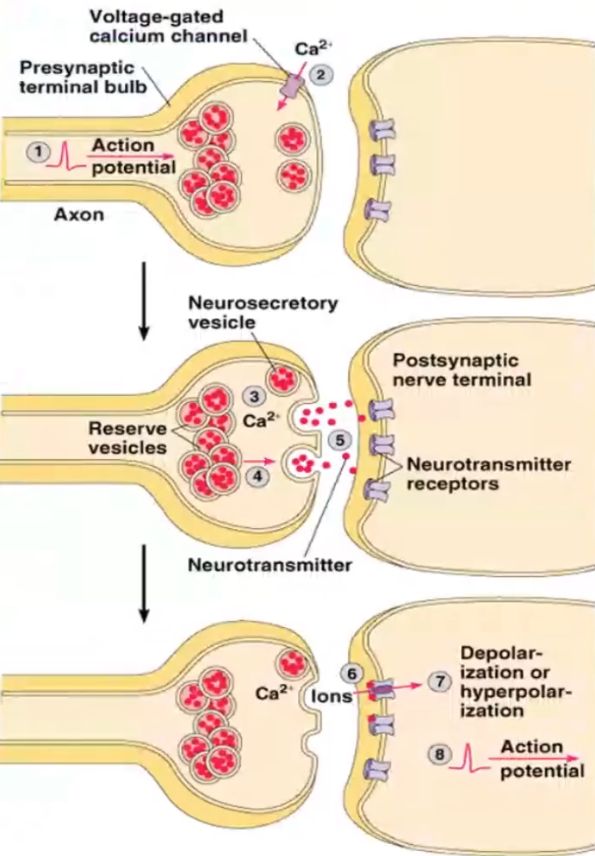
\includegraphics[width=0.7\textwidth]{neurotransmission}
    \caption{Action potential in presynaptic neuron releases neurotransmitters that pump \ce{Na+} into postsynaptic neuron, effectively transmitting the action potential across the gap (at this level, ignore the rest, such as calcium)}
\end{figure}

\subsubsection{Examples}
\begin{itemize}
    \item{\textbf{Acetylcholine} = usually excitatory: opens \ce{Na+} channels, causing depolarization}
    \item{\textbf{Cholinesterase} = enzyme in synapse; destroys acetylcholine, ending depolarization to avoid getting stuck; \\ acetylcholine return to presynaptic neuron to be stored}
    \item{Acetylcholine may act as inhibitory: opening \ce{K+} gates and diffusing \ce{K+} out of neuron, causing hyperpolarization}
\end{itemize}

You do not need to memorize these.
\begin{figure}[H]
    \centering
    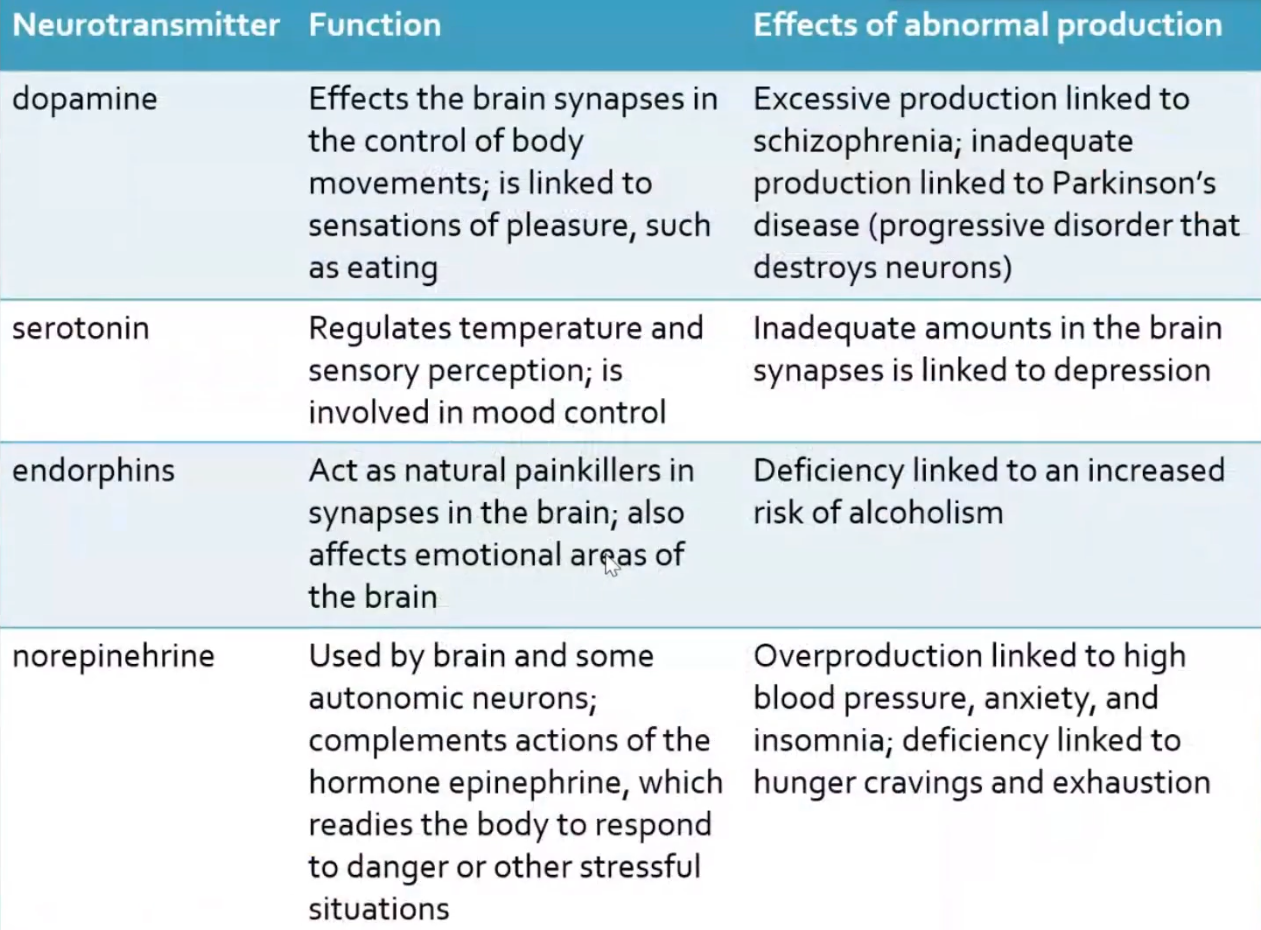
\includegraphics[width=\textwidth]{transex}
\end{figure}

\section{Summation}
\begin{itemize}
    \item{Multiple neurons required to stimulate another neuron}
    \item{\hl{Sum} of multiple action potentials to \hl{reach the threshold} of another}
\end{itemize}
\begin{figure}[H]
    \centering
    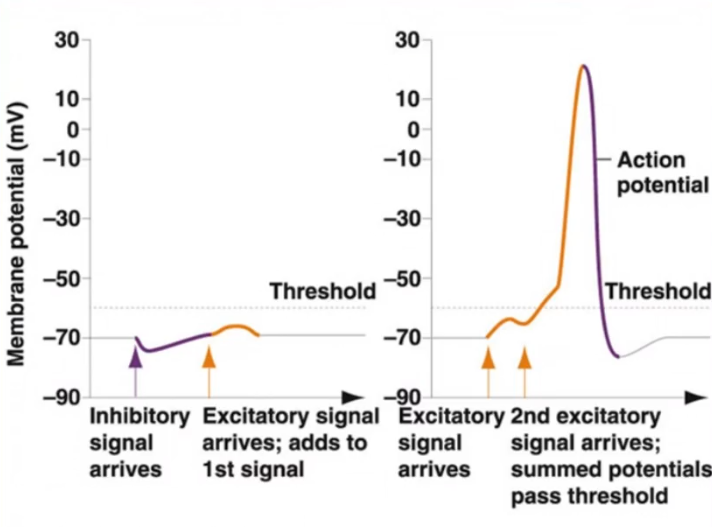
\includegraphics[width=0.6\textwidth]{summation}
\end{figure}

\section{(13.3) Central Nervous System}

\subsection{Spinal Cord}
\begin{itemize}
    \item{Tube-like organ of neurons, glial cells, and blood vessals}
    \item{Located inside of backbone or spine}
    \item{Carries sensory nerve messages from receptors to brain (interneurons)}
    \item{Relays motor nerve messages from brain to muscles and glands}
    \item{\textbf{Central canal} = contains CSF}
\end{itemize}

\subsection{The Brain}
\begin{itemize}
    \item{Coordinating center of nervous system}
    \item{Enclosed within skull}
    \item{\textbf{Meninges} = \hl{3 protective membranes} surrounding the brain, fluid within}
    \item{\textbf{Meningitis} = bacterial or viral \hl{infection} of any of the outer membranes of the brain}
    \item{
            \textbf{Cerebrospinal fluid (CSF)} = nourishing fluid, shock absorber; \\ found within...
            \begin{itemize}
                \item{inner and middle layer of meninges}
                \item{through central canal of spinal cord}
            \end{itemize}
        }
    \item{More nerve tracts in mouth, face and hands, compared to legs and arms}
\end{itemize}

\begin{figure}[H]
    \centering
    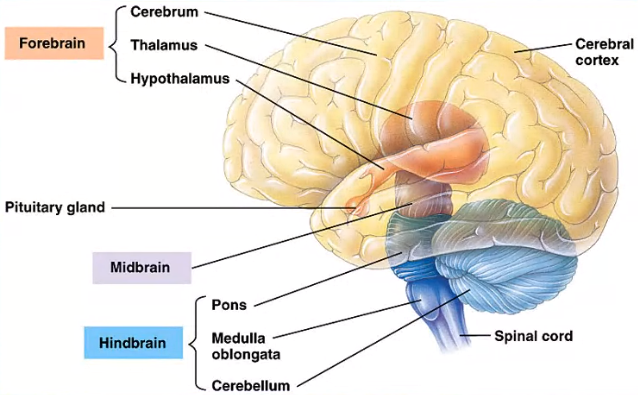
\includegraphics[width=\textwidth]{brains}
\end{figure}


\section{Forebrain}
\begin{itemize}
    \item{\textbf{Forebrain} = reason, intellect, memory, language, personality}
    \item{\textbf{Cerebrum} = largest portion of brain}
    \item{\textbf{Cerebral cortex} = surface of cerebrum, gray matter (unmyelinated)}
    \item{Coordinating center for motor actions, speech, reasoning, memory, personality}
\end{itemize}

\subsection{Hemispheres}
\begin{figure}[H]
    \centering
    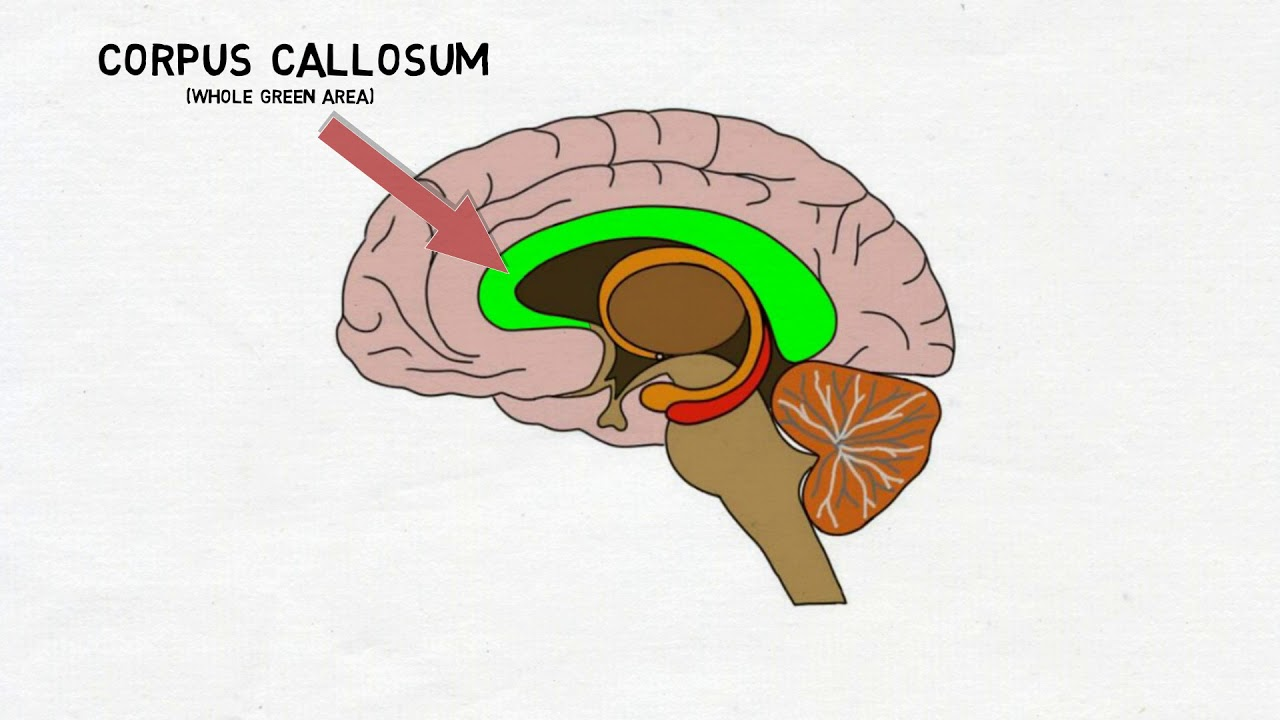
\includegraphics[width=0.50\textwidth]{corpus}
\end{figure}
\begin{itemize}
    \item{\textbf{Corpus callosum} = communication bridge between left and right brain}
    \item{
            2 distinct hemispheres
            \begin{itemize}
                \item{\hl{Left = verbal skills}}
                \item{\hl{Right = visual patterns and spatial awareness}}
            \end{itemize}
            \begin{figure}[H]
                \centering
                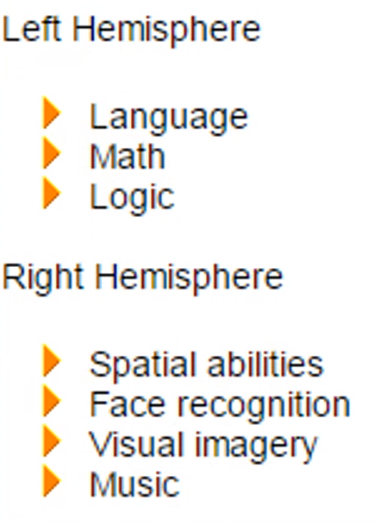
\includegraphics[width=0.2\textwidth]{hemi}
            \end{figure}
        }
    \item{\textbf{Severed corpus callosum} = impairment of memory, walking, balance}
\end{itemize}
\subsubsection{Left Hemisphere}
\begin{itemize}
    \item{\textbf{Stroke} = if left side, speech may be lost}
    \item{\textbf{Broca's area} = production of language; tongue, lips, and jaw motion}
    \item{\textbf{Wernicke's area} = processing of spoken words, interpreting emotions}
\end{itemize}

\subsection{Cerebrum Lobes}
\begin{figure}[H]
    \centering
    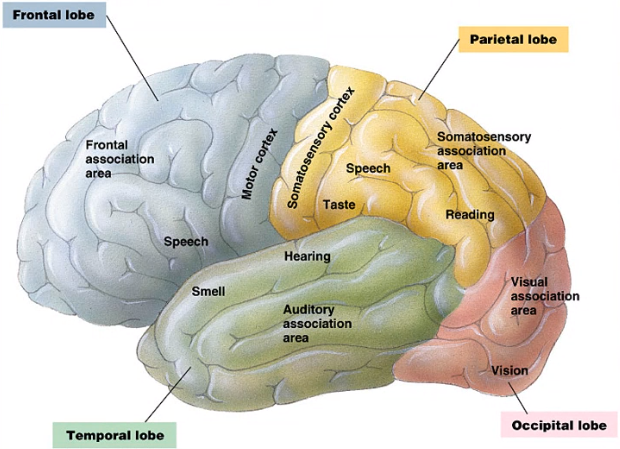
\includegraphics[width=\textwidth]{lobes}
\end{figure}
\begin{itemize}
    \item{Each hemisphere has 4 lobes}
    \item{
            \textbf{Frontal}
            \begin{itemize}
                \item{\hl{voluntary muscles} (walking, speech)}
                \item{\hl{personality}, knowing right from wrong}
                \item{\hl{memory (IQ)}}
            \end{itemize}
        }
    \item{
            \textbf{Temporal}
            \begin{itemize}
                \item{interpret sensory info (hearing, smell, \emph{some} vision)}
                \item{\hl{sound and smell memory}}
                \item{\textbf{Amygdala} = found near hearing centre of brain, associated with memory}
            \end{itemize}
        }
    \item{
            \textbf{Parietal}
            \begin{itemize}
                \item{\hl{touch (temperature awareness), taste, pain}}
                \item{emotions}
                \item{interpreting speech}
                \item{Wernicke's area}
            \end{itemize}
        }
    \item{
            \textbf{Occipital}
            \begin{itemize}
                \item{\hl{vision}}
            \end{itemize}
        }
\end{itemize}

\subsection{Thalamus}
\begin{itemize}
    \item{Interprets and distributes sensory information}
    \item{Sensory info. such as smell, taste, touch, vision, sound}
    \item{\hl{Redirects} messages from spinal cord to \hl{appropriate lobes} of the brain}
    \item{Relay station, like a post office}
\end{itemize}

\subsection{Hypothalamus \& Pituitary Gland}
\begin{itemize}
    \item{Unites nervous and endocrine systems (autonomic functions)}
    \item{\hl{Regulates internal environment} (maintains body temp)}
    \item{Notifies thirst and hunger}
    \item{\textbf{Pituitary Gland} = master gland, related to hormones and stress}
\end{itemize}

\subsection{Olfactory Bulbs}
\begin{itemize}
    \item{Detects smell}
    \item{
            Pathway (nr test question)
            \begin{itemize}
                \item{Odor molecule dissolved in mucus}
                \item{AP occurs (depolarization)}
                \item{Sent to temporal lobe}
            \end{itemize}
        }
\end{itemize}

\subsection{Limbic System}
\begin{figure}[H]
    \centering
    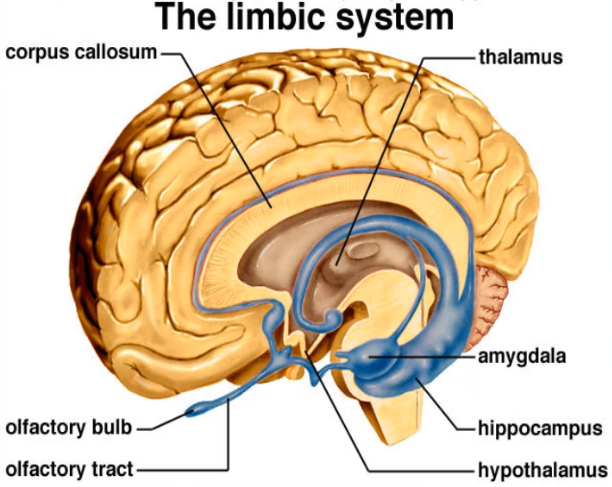
\includegraphics[width=0.50\textwidth]{limbic}
    \caption{Limbic system is in blue}
\end{figure}
\begin{itemize}
    \item{Influences ANS and endocrine system}
    \item{
            Interconnected with...
            \begin{itemize}
                \item{\hl{healthy concious state of mind} (confidence)}
                \item{pleasure centre}
                \item{emotions}
                \item{memory}
            \end{itemize}
        }
\end{itemize}

\section{Midbrain}
\begin{itemize}
    \item{Acts as a relay center for some, not all, \hl{eye and ear} reflexes}
    \item{Less developed than forebrain}
    \item{Consisting of 4 spheres of gray matter}
\end{itemize}

\begin{figure}[H]
    \centering
    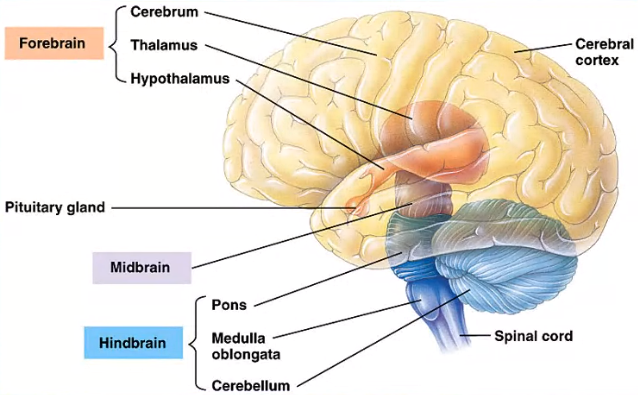
\includegraphics[width=0.7\textwidth]{brains}
\end{figure}

\section{Hindbrain}
\begin{itemize}
    \item{\textbf{Hindbrain} = balance, muscle control, autonomic control}
    \item{Found behind midbrain, joins with spinal cord}
\end{itemize}

\subsection{Cerebellum}
\begin{itemize}
    \item{Located immediately beneath the 2 cerebral hemispheres}
    \item{Largest section of hindbrain}
    \item{\hl{Fine and major} limb movements, \hl{balance}, muscle tone}
\end{itemize}

\subsection{Pons}
\begin{itemize}
    \item{
            A bridge/relay station that passes info between
            \begin{itemize}
                \item{the 2 regions of the cerebellum}
                \item{between the cerebellum and the medulla}
            \end{itemize}
        }
\end{itemize}

\subsection{Medulla Oblongata}
\begin{itemize}
    \item{Posterior region of hindbrain, aka. brain stem}
    \item{Acts as a connection between PNS and CNS}
    \item{Coordinating center for ANS (\hl{breathing, heart rate}, peristalsis, blood pressure)}
    \item{Connected directly to spinal cord}
\end{itemize}

\section{Brain Mapping}
\begin{itemize}
    \item{\textbf{Phrenology} = false science, feel bumps on head to figure out things}
\end{itemize}

\section{Drugs}
\begin{itemize}
    \item{\textbf{Endorphins} = attach to neurons in CNS, preventing production of pain transmitters}
    \item{\textbf{Euphoria} = tranquility feeling produced by endorphins; pain killers, opiates, heroin, codeine, morphine act the same way as endorphins}
    \item{When drug usage stop, pain transmitter is produced in abundance; "fake" pain}
    \item{\textbf{Barbiturates} = sleeping pills}
\end{itemize}

\section{Alzheimer's Disease}
\begin{itemize}
    \item{Progressive, degenerative neurological disease}
    \item{Linked with aging}
    \item{Deterioration of thinking and of memory}
    \item{Production of plaques and tangles}
    \item{
            \textbf{Plaques}
            \begin{itemize}
                \item{In healthy brains, beta amyloid protein deposits exist}
                \item{In Alzheimer's patients, secretases work too well, produce too much beta amyloid}
                \item{Affect neurons}
            \end{itemize}
        }
    \item{
            \textbf{Tangles}
            \begin{itemize}
                \item{Healthy neurons grow and behave abnormally}
                \item{Choke and kill neuron}
            \end{itemize}
        }
\end{itemize}
\begin{figure}[H]
    \centering
    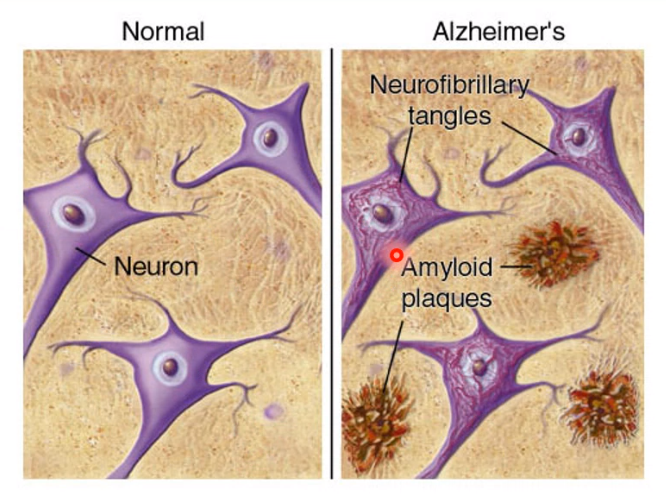
\includegraphics[width=0.50\textwidth]{alz}
\end{figure}

\section{(13.4) Peripheral Nervous System}
\begin{figure}[H]
    \centering
    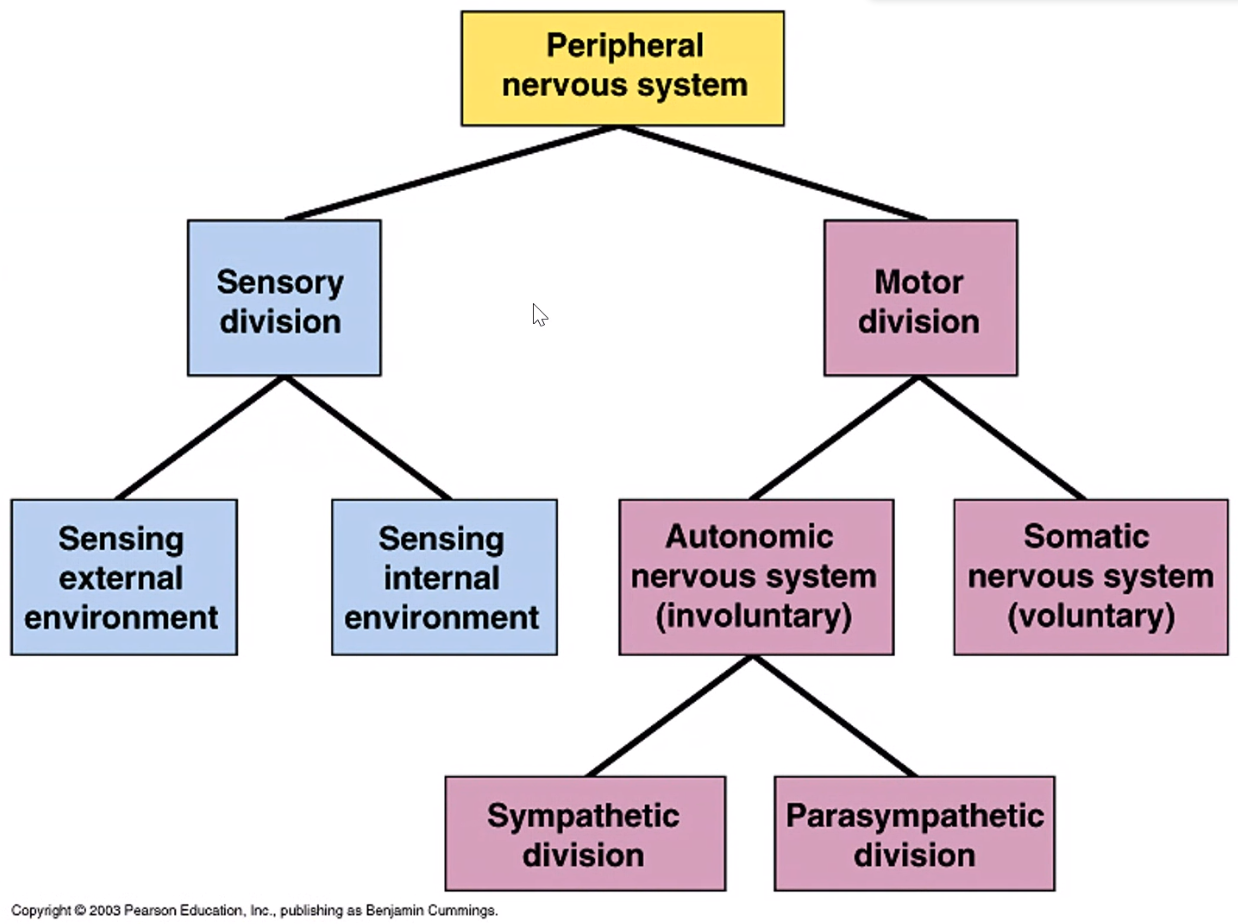
\includegraphics[width=0.75\textwidth]{peripheral}
\end{figure}
\begin{itemize}
    \item{\textbf{Autonomic system} = nerves designed to \hl{maintain internal homeostasis} (involuntary)}
    \item{\textbf{Somatic system} = nerves designed to \hl{adjust to external stimuli} by controlling skeletal muscle (voluntary, exception: reflexes)}
\end{itemize}

\subsection{Somatic Sensory System}
\begin{itemize}
    \item{Brings info from external environment, CNS, skeletal muscles}
    \item{Voluntary control}
    \item{Reflex arcs are involuntary, but still categorized as somatic}
\end{itemize}

\subsection{Autonomic Nervous System}
\begin{itemize}
    \item{\hl{Involuntary internal homeostatic control}}
    \item{\textbf{Autonomic nerves} = motor nerves, regular organs of body involuntarily}
\end{itemize}

\begin{figure}[H]
    \centering
    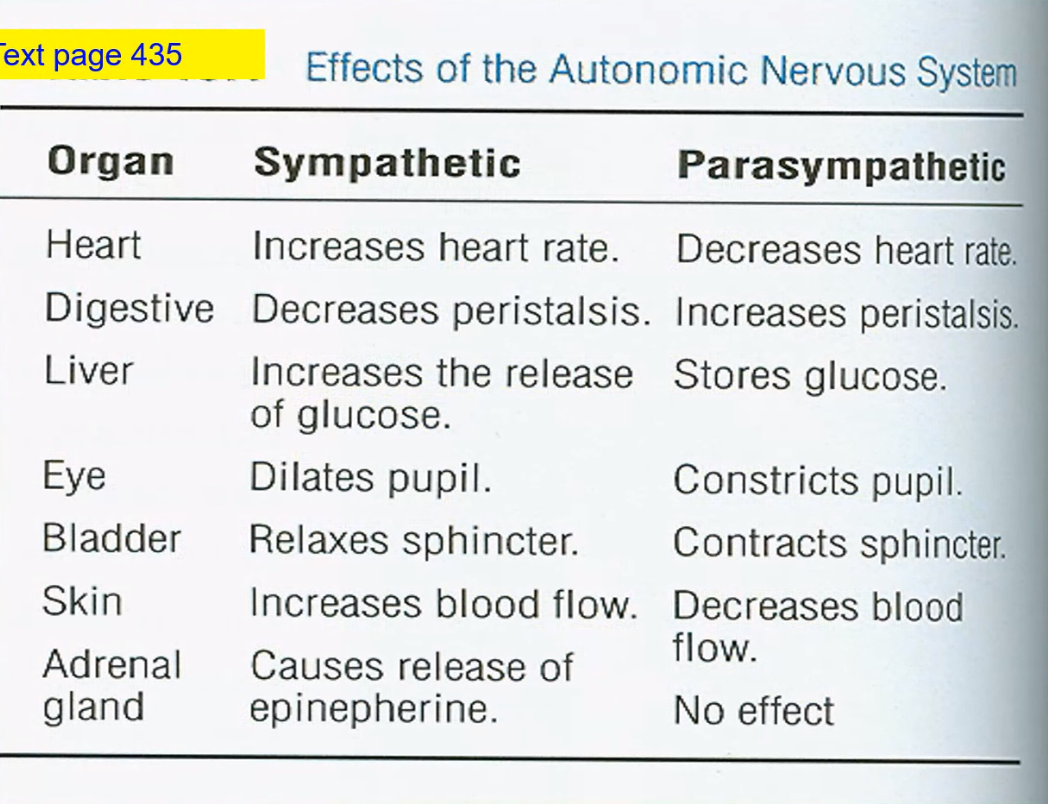
\includegraphics[width=0.40\textwidth]{symandpara}
\end{figure}

\subsubsection{Sympathetic}
\begin{figure}[H]
    \centering
    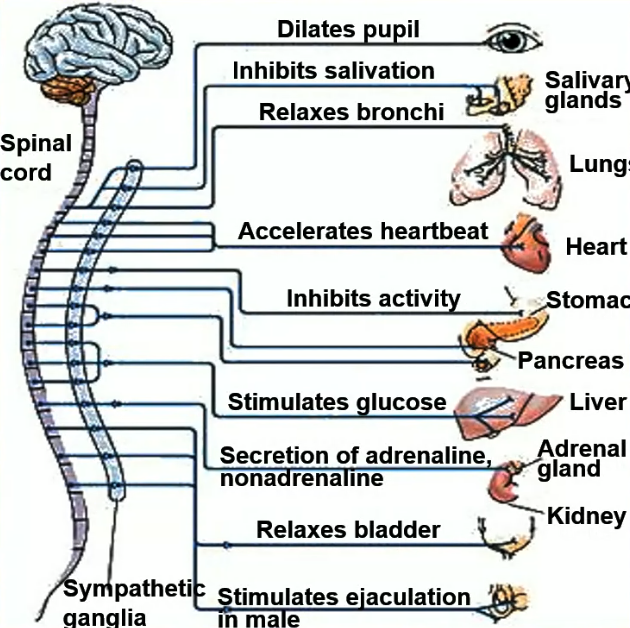
\includegraphics[width=0.50\textwidth]{sympathetic}
\end{figure}
\begin{itemize}
    \item{Prepares body for stress \\ \textbf{'Fight, flight, or freeze'} response}
    \item{Releases adrenaline and noradrenaline --- both hormones do the same thing}
    \item{
            Excitatory in...
            \begin{itemize}
                \item{increases heart rate and blood pressure}
                \item{increases blood flow to skeletal muscles}
                \item{etc... (diagram)}
            \end{itemize}
        }
    \item{
            Inhibitory in...
            \begin{itemize}
                \item{inhibits digestive functions}
                \item{etc... (diagram)}
            \end{itemize}
        }
\end{itemize}

\subsubsection{Parasympathetic}
\begin{figure}[H]
    \centering
    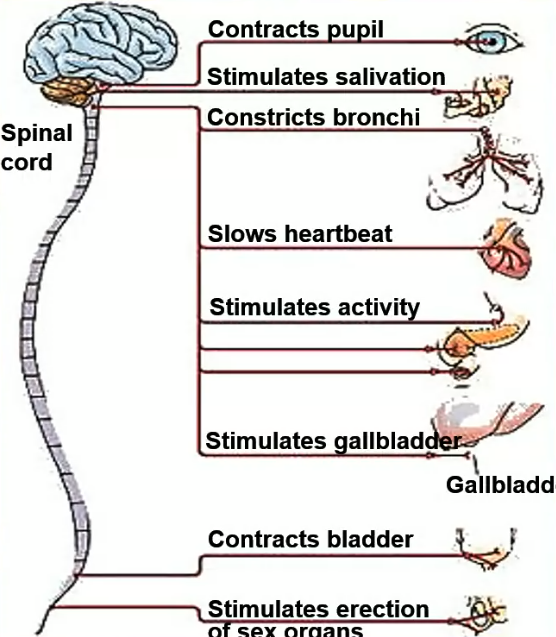
\includegraphics[width=0.50\textwidth]{parasympathetic}
\end{figure}
\begin{itemize}
    \item{Restores balance in body \\ \textbf{'Rest and digest'} response}
    \item{Calms body to conserve and maintain energy}
    \item{Lowers heartbeat, breathing rate, blood pressure}
\end{itemize}

\subsection{Vagus Nerve}

\section{(14.1) Senses}
\begin{itemize}
    \item{\textbf{Stimulus} = source of energy converted from one form to another}
    \item{\textbf{Sensory receptors} (dendrites of sensory neurons) = \\ convert one energy form (info) about the external environment \\ into electrochemical energy (nerve impulses, aka. action potentials) \\ that are then relayed to the CNS}
    \item{Each individual receptor is capable of responding to \hl{only one kind of stimulus}}
    \item{Stimulation of grouped receptors results in \hl{only one type of sensation} \\ ex. eye (light receptor) = sight}
    \item{Grouped receptors help reach threshold levels}
    \item{\textbf{Sensory adaptation} = constant exposure to a certain stimulus leads to an \hl{insensitivity} of the sensory receptor to said stimulus \\ ex. don't notice smell of your home}
\end{itemize}

\subsection{Receptors}
\begin{itemize}
    \item{
            \textbf{Photoreceptors}
            \begin{itemize}
                \item{eyes (rods, cones)}
            \end{itemize}
        }
    \item{
            \textbf{Chemoreceptors}
            \begin{itemize}
                \item{tongue (taste buds, 50-100 neurons) \\ salty, sweet, sour, bitter, umami (savoury)}
                \item{nose (olfactory cells) \\ airbourne chemicals detected by olfactory cells of olfactory bulb, connected to temporal lobe}
                \item{carotid arteries \& brain (blood pH)}
            \end{itemize}
        }
    \item{
            \textbf{Mechanoreceptors}
            \begin{itemize}
                \item{ear (inner-ear hair cells, balance, sound)}
                \item{touch and pressure (skin)}
                \item{\textbf{Proprioceptors} (skin, muscles) = interpret movement/position of limbs in space and time (without just looking)}
            \end{itemize}
        }
    \item{
            \textbf{Thermoreceptors}
            \begin{itemize}
                \item{heat \& cold (skin)}
            \end{itemize}
        }
\end{itemize}

\begin{figure}[H]
    \centering
    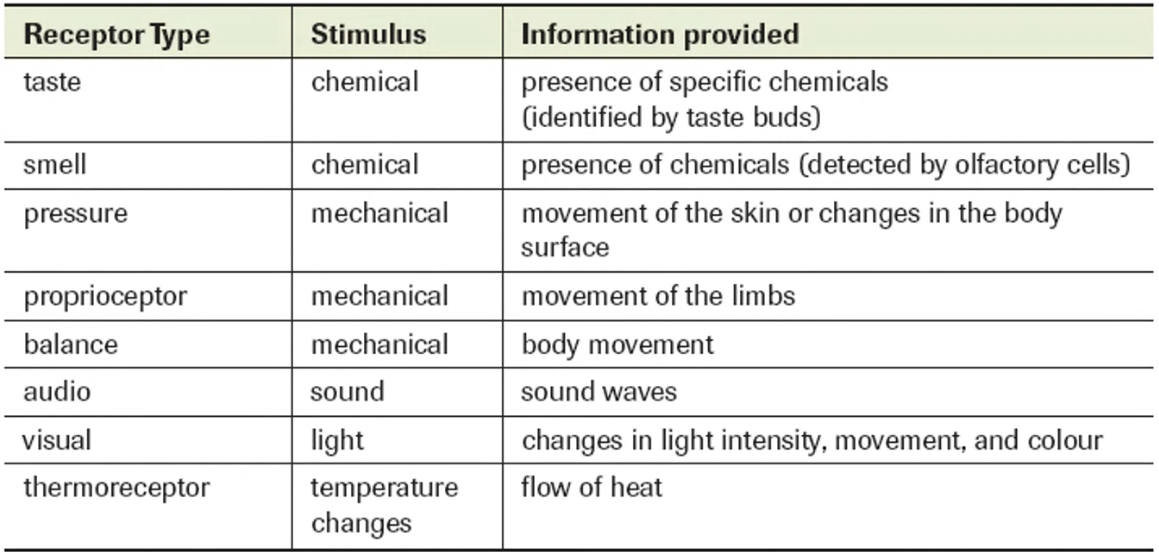
\includegraphics[width=0.75\textwidth]{sense-summary}
\end{figure}

\pagebreak

\section{(14.2) Photoreception}

\begin{figure}[H]
    \centering
    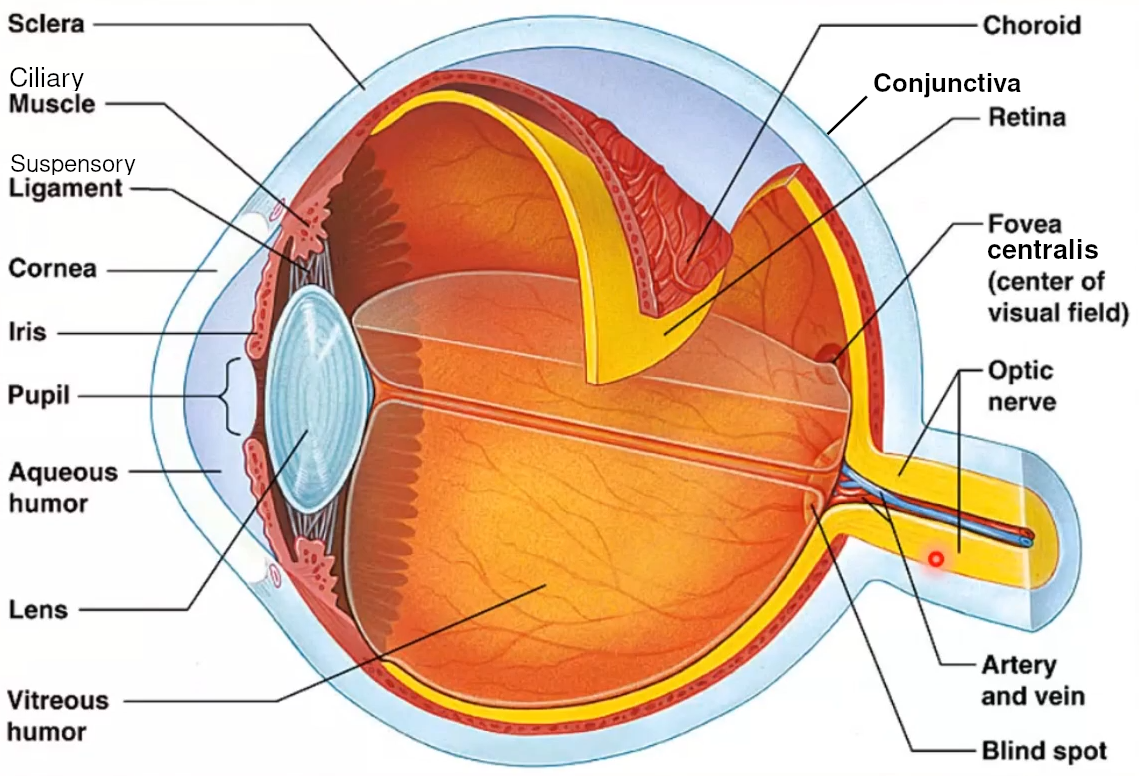
\includegraphics[width=\textwidth]{eye}
\end{figure}

\subsection{Sclera}
\begin{itemize}
    \item{\hl{white}, fibrous outermost layer of eye}
    \item{protective layer}
    \item{maintains eye's shape}
    \item{\textbf{Conjunctiva} = covers outer surface of sclera, \hl{does not cover cornea}, \hl{keeps eye moist}}
\end{itemize}

\subsubsection{Cornea}
\begin{itemize}
    \item{\hl{front of sclera} covered in window-like cornea, \hl{bends light toward pupil}}
    \item{requires oxygen and nutrients}
    \item{not supplied with blood vessels}
\end{itemize}

\subsubsection{Aqueous humor}
\begin{itemize}
    \item{\hl{Anterior}, space behind cornea}
    \item{supplies \hl{nutrients to cornea}}
    \item{blinking and tears resupplies oxygen in aqueous humor}
\end{itemize}

\subsection{Choroid Layer}
\begin{itemize}
    \item{middle layer of eye, contains blood vessels}
    \item{pigmented black to \hl{prevent light scattering}}
\end{itemize}

\subsubsection{Iris}
\begin{itemize}
    \item{thin circular muscle}
    \item{controls the \hl{size of pupil} opening}
\end{itemize}

\subsubsection{Lens}
\begin{itemize}
    \item{\hl{focuses image on retina}, behind iris}
    \item{cornea still does most of light bending}
\end{itemize}

\subsubsection{Ciliary Muscles}
\begin{itemize}
    \item{internal/intrinsic}
    \item{attached to ligaments}
    \item{\hl{indirectly} alter shape of lens}
    \item{\hl{focus far/near}}
\end{itemize}

\subsubsection{Vitreous Humor}
\begin{itemize}
    \item{large chamber behind lens}
    \item{cloudy, jellylike material}
    \item{\hl{maintains shape} of eyeball}
    \item{permits \hl{light transmission} to retina}
\end{itemize}

\subsection{Retina}
\begin{figure}[H]
    \centering
    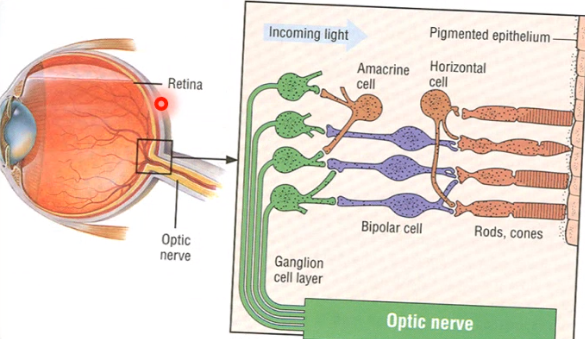
\includegraphics[width=0.75\textwidth]{retina}
\end{figure}
\begin{itemize}
    \item{innermost layer of eye}
    \item{
            \hl{Action potential pathway}
            \begin{itemize}
                \item{light-sensitive cells (rods, cones)}
                \item{bipolar cells}
                \item{cells of optic nerve}
                \item{CNS}
            \end{itemize}
        }
\end{itemize}

\subsection{Photoreceptor Cells}
\begin{itemize}
    \item{sensory neurons}
    \item{in light-sensitive layer, next to choroid layer}
\end{itemize}

\subsubsection{Rods}
\begin{itemize}
    \item{extremely sensitive --- single photon can stimulate}
    \item{respond to low-intensity light}
    \item{more rods than cons}
    \item{only black and white}
    \item{detect motion, make up peripheral vision}
    \item{concentrated in outside edges of retina}
\end{itemize}

\subsubsection{Cones}
\begin{itemize}
    \item{respond to intense light (red, green, blue)}
    \item{eye must focus light onto the fovea centralis to produce a sharp image}
    \item{concentrated at fovea centralis --- back and center of retina}
    \item{allows high acuity tasks, such as reading}
    \item{\textbf{Color Blindness} = lack or deficiency in particular cones, usually green and red, sex-linked}
\end{itemize}

\subsection{Spots}
\subsubsection{Fovea centralis}
\begin{itemize}
    \item{Depression in retina, center of vision}
    \item{High concentration of cones, \hl{no rods}}
    \item{Most sensitive area of eye}
    \item{Most light rays fall on fovea centralis}
\end{itemize}

\subsubsection{Blind Spot}
\begin{itemize}
    \item{aka. Optic disc}
    \item{Where ganglion cells merge to \hl{form the optic nerve}}
    \item{\hl{No rods or cones}}
\end{itemize}

\section{Visual Interpretation}
\begin{itemize}
    \item{Occipital lobe processes info from each photoreceptor neuron}
    \item{\hl{Flips image right-side up}}
\end{itemize}

\subsection{[IB] Crossing}

\begin{figure}[H]
    \centering
    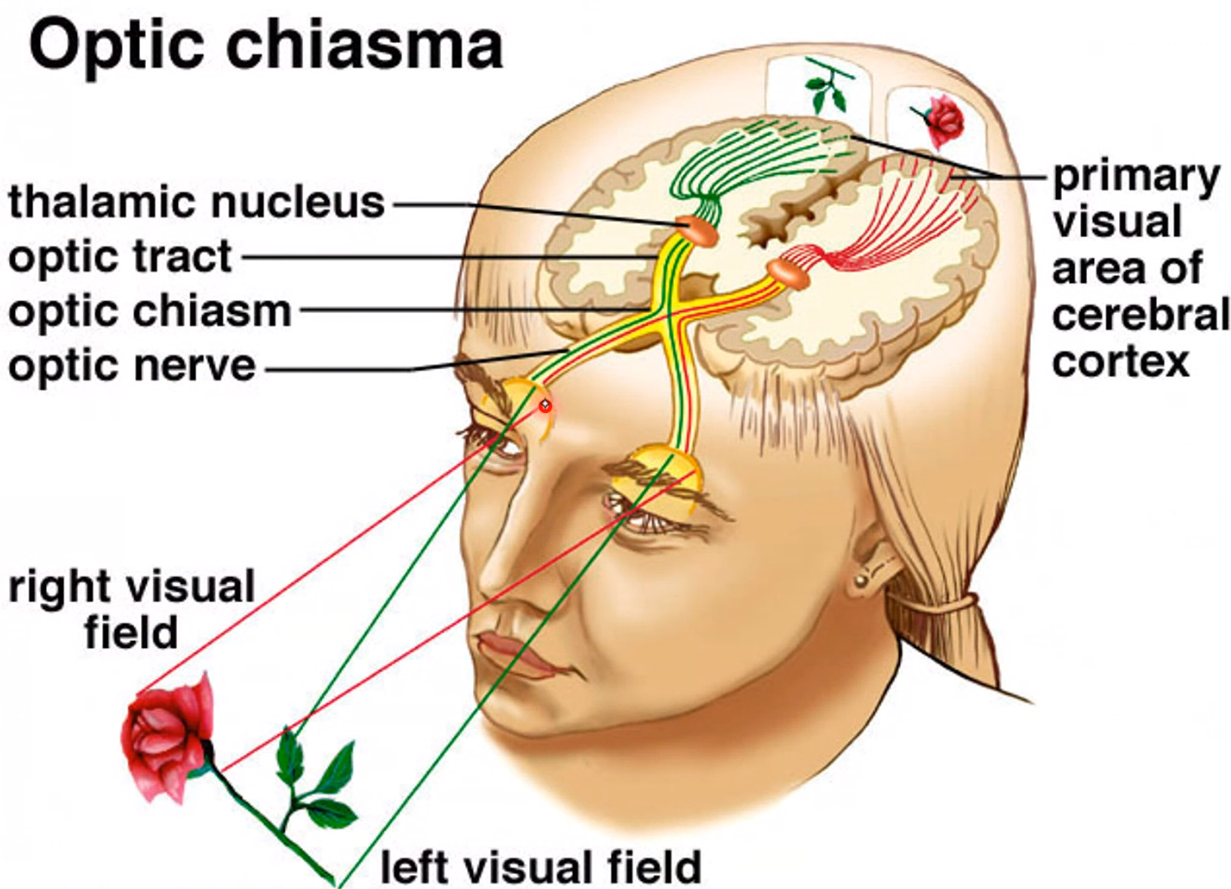
\includegraphics[width=0.50\textwidth]{cross}
\end{figure}

Objects on one side of your vision are interpretated by the opposing side of your brain (object on right, left brain) but both eyeballs capture light of said object, with the neural information crossing paths

\subsection{Accommodation}
Ability to change lens shape in order to focus.

\subsubsection{Far Away}
\begin{figure}[H]
    \centering
    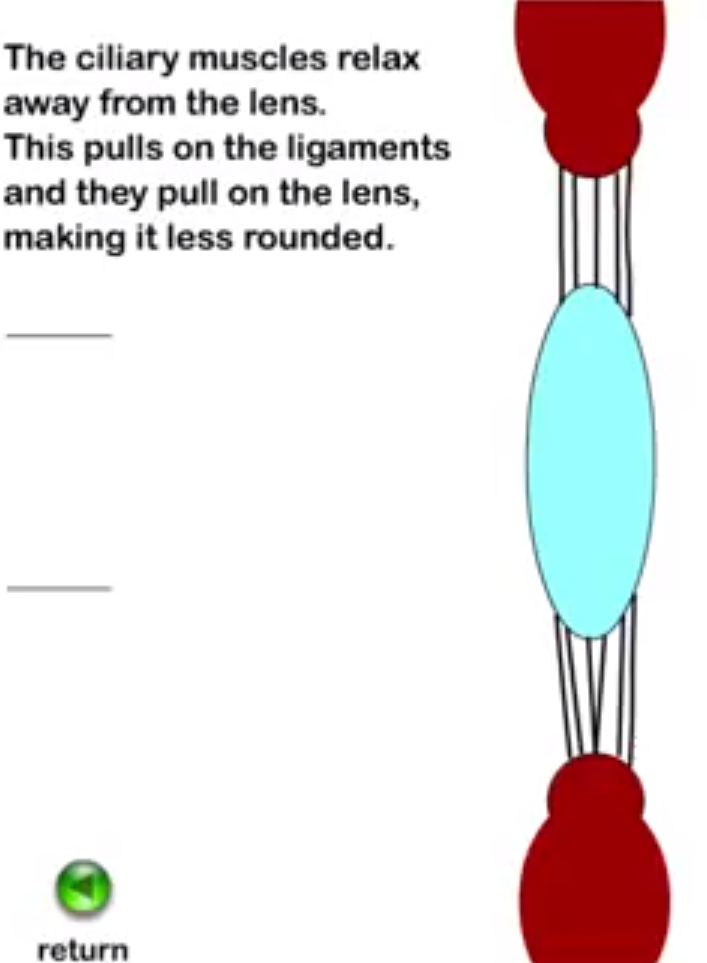
\includegraphics[width=0.50\textwidth]{far}
\end{figure}
\begin{itemize}
    \item{
            \hl{Lens thins}
            \begin{itemize}
                \item{Ciliary muscles relax, away from lens}
                \item{Suspensory ligaments become tight (tension from ligaments)}
                \item{Lens flattens}
                \item{Pupil dilates}
            \end{itemize}
        }
\end{itemize}

\subsubsection{Close Up}
\begin{figure}[H]
    \centering
    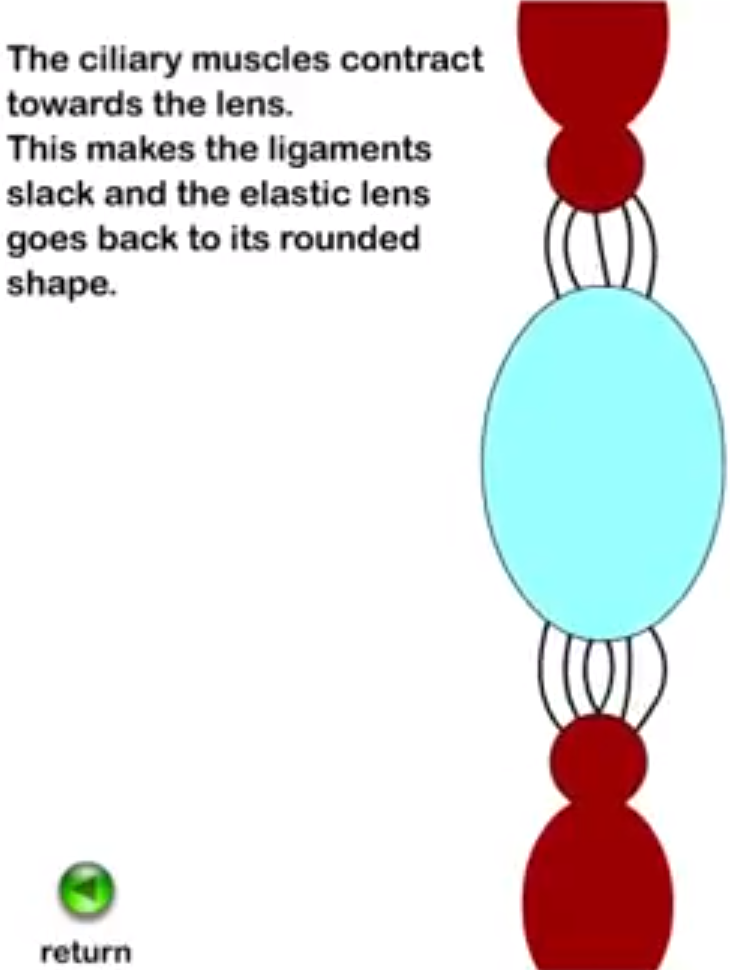
\includegraphics[width=0.50\textwidth]{close}
\end{figure}
\begin{itemize}
    \item{
            \hl{Lens thickens}
            \begin{itemize}
                \item{Ciliary muscles contract, towards lens}
                \item{Suspensor ligaments relax}
                \item{Lens becomes rounded}
                \item{Pupil constricts}
            \end{itemize}
        }
\end{itemize}

\subsection{Defects}
\subsubsection{Astigmatism}
\begin{figure}[H]
    \centering
    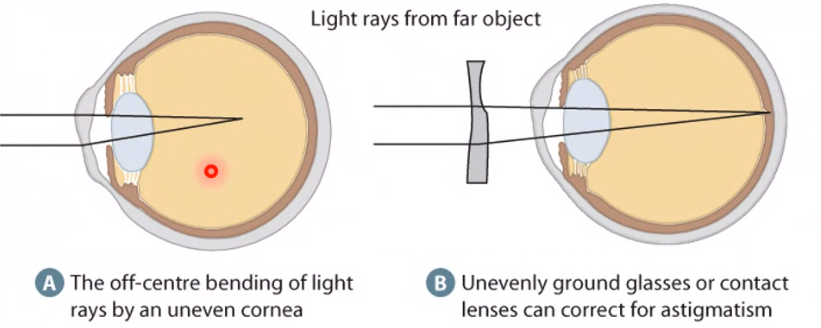
\includegraphics[width=0.75\textwidth]{astigmatism}
    \caption{Uneven curvature of part of the cornea, treated with glasses}
\end{figure}

\subsubsection{Cataracts}
\begin{figure}[H]
    \centering
    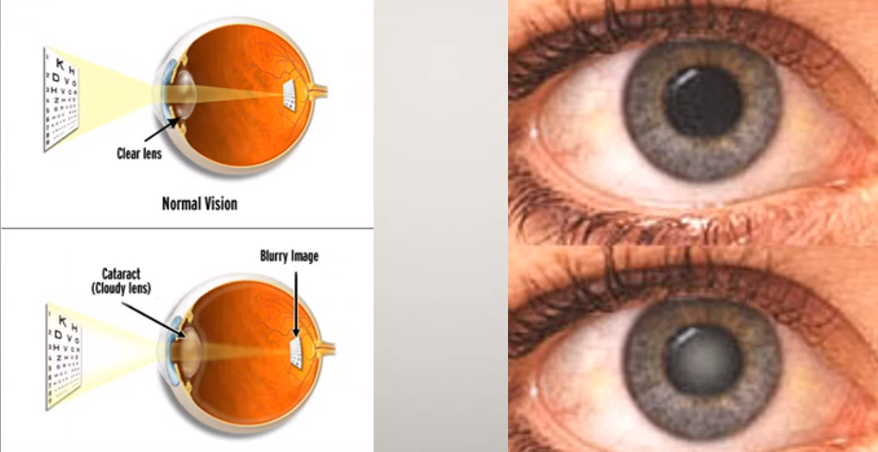
\includegraphics[width=\textwidth]{cataracts}
    \caption{Lens becomes opaque, treated with glasses or new lens}
\end{figure}

\subsubsection{Glaucoma}
\begin{figure}[H]
    \centering
    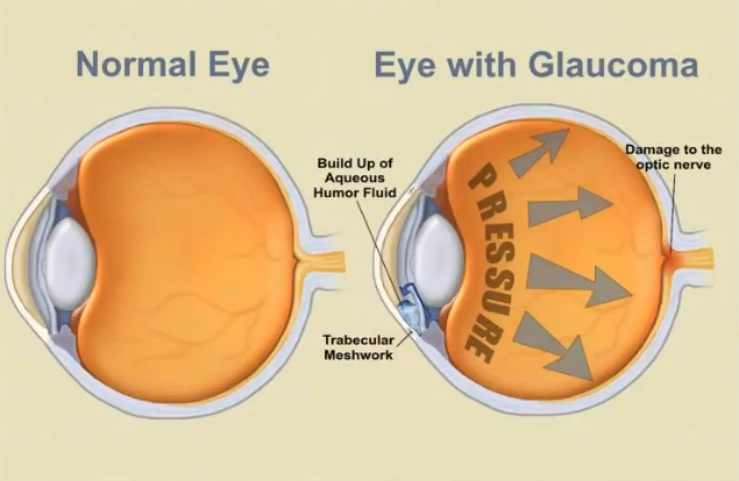
\includegraphics[width=0.75\textwidth]{glaucoma}
    \caption{Build-up of fluid in aqueous humor, creating pressure, damaging the optic nerve}
\end{figure}

\subsubsection{Colour Blindness}
\begin{itemize}
    \item{Inherited condition}
    \item{Lacking certain cones (red, green, or blue)}
\end{itemize}

\subsubsection{Myopia}
\begin{figure}[H]
    \centering
    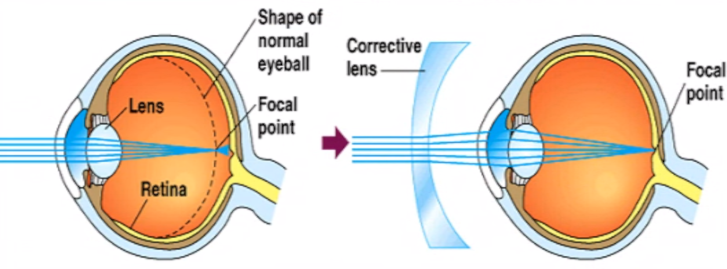
\includegraphics[width=0.50\textwidth]{myopia}
\end{figure}
\begin{itemize}
    \item{Near-sighted}
    \item{Cannot focus on objects far away, only close up}
    \item{Elongated eyeball}
    \item{Focused image falls \hl{in front of retina}}
    \item{Corrected with \hl{concave lenses}}
\end{itemize}

\subsubsection{Hyperopia}
\begin{figure}[H]
    \centering
    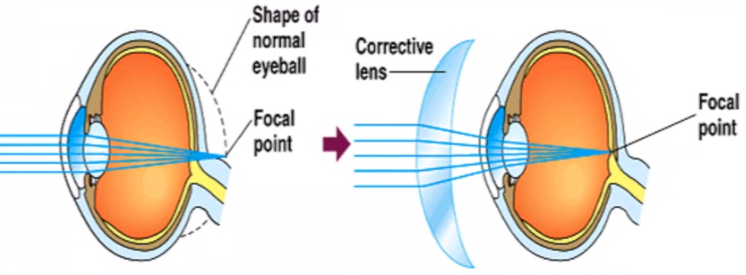
\includegraphics[width=0.50\textwidth]{hyperopia}
\end{figure}
\begin{itemize}
    \item{Far-sighted}
    \item{Cannot focus on objects close up, only far away}
    \item{Eyeball too short}
    \item{Focused image falls \hl{behind of retina}}
    \item{Corrected with \hl{convex lenses}}
\end{itemize}

\pagebreak

\section{[IB] Chemistry of Vision}
\begin{itemize}
    \item{\textbf{Rhodopsin} = light pigment found in rods}
    \item{\textbf{Photopsin} = colour pigment found in cones}
\end{itemize}

\subsection{Rhodopsin/Photopsin Pathaway}
\begin{figure}[H]
    \centering
    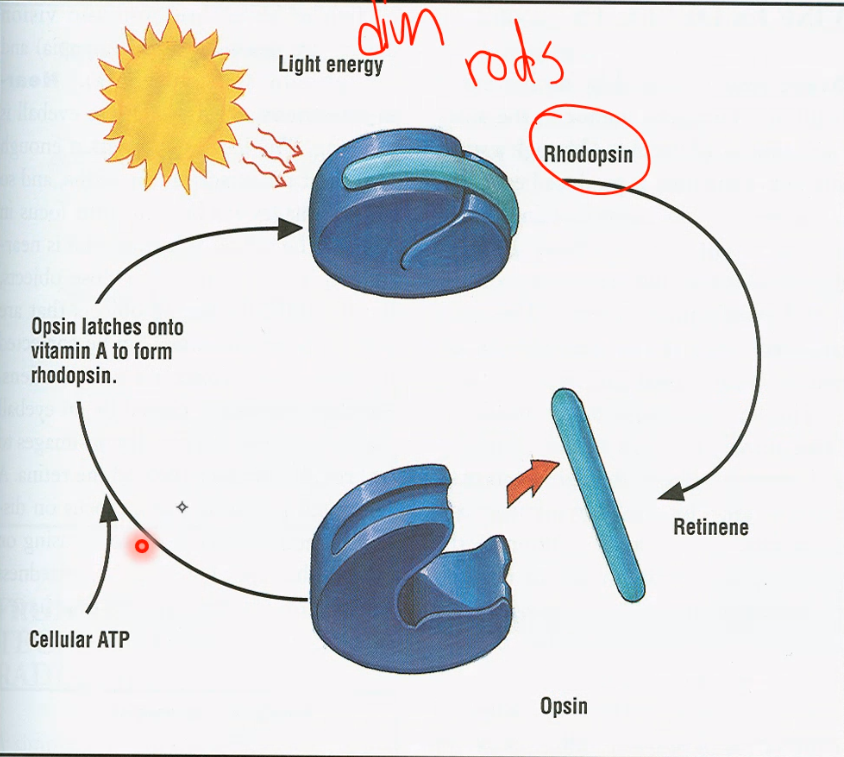
\includegraphics[width=0.75\textwidth]{rhodopsin}
\end{figure}
\begin{itemize}
    \item{Rods absorb dim light}
    \item{Rhodopsin splits into \textbf{retinal} (vitamin A derivative) and protein \textbf{opsin}}
    \item{Triggers a chain reaction}
    \item{\hl{Stops release of inhibitory neurostransmitter molecules}}
    \item{Allows \hl{action potential} to occur to optic nerve}
    \item{Similar process occurs for cones, except with photopsin}
\end{itemize}

\subsection{Pathway through Retina Layers}
\begin{figure}[H]
    \centering
    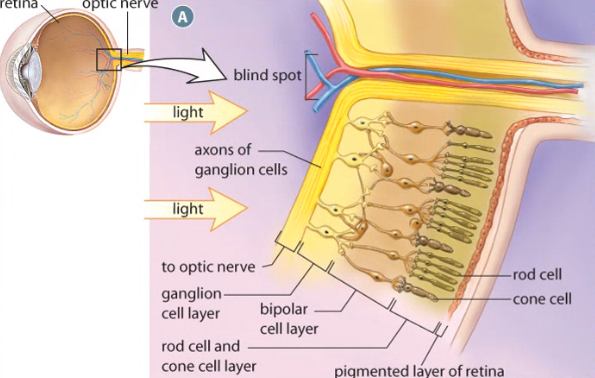
\includegraphics[width=0.75\textwidth]{retina-pathway}
\end{figure}
\begin{itemize}
    \item{\hl{Light rays pass through several layers of retina}}
    \item{Reach and trigger rods and cones \hl{first}}
    \item{Rods/cones have synapse with bipolar cells, middle layer}
    \item{Bipolar cells transfer action potential to ganglion cells, deepest layer}
    \item{Ganglion cells form optic nerve}
\end{itemize}

\pagebreak

\section{(14.3) Ear}
\begin{figure}[H]
    \centering
    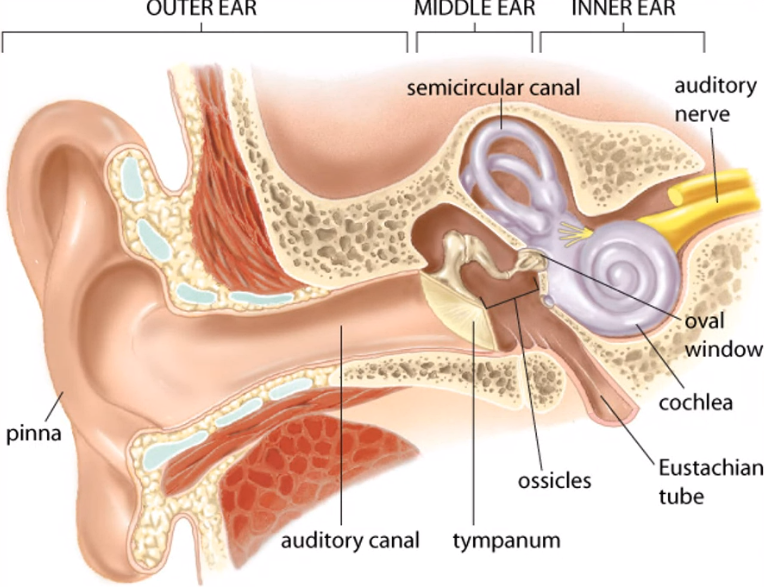
\includegraphics[width=\textwidth]{ear}
\end{figure}

\subsection{Outer Ear}

\subsubsection{Pinna}
\begin{itemize}
    \item{Composed of cartilage}
    \item{Shaped to funnel sound waves into auditory canal}
\end{itemize}

\subsubsection{Auditory Canal}
\begin{itemize}
    \item{Channel carrying sound waves to ear drum}
    \item{
            Consists of cells that
            \begin{itemize}
                \item{grow hair to catch dust}
                \item{produce mucus to form ear wax, which trap particles}
            \end{itemize}
        }
\end{itemize}

\pagebreak

\subsection{Middle Ear}

\subsubsection{Tympanic Membrane}
\begin{itemize}
    \item{aka. tympanum, ear drum}
    \item{Vibrates from sound waves}
\end{itemize}

\subsubsection{Ossicles}
\begin{itemize}
    \item{3 bones, smallest bones of your body}
    \item{\hl{Concentrate and amplify} vibrations from tympanic membrane}
    \item{Held together by muscles and ligaments}
    \item{Muscles protect inner ear against excessive noise}
\end{itemize}

\subsubsection{Oval Window}
\begin{itemize}
    \item{Smaller than eardrum}
    \item{Receives vibrations from ossicles}
    \item{Triggers waves of fluid within inner ear}
\end{itemize}

\subsubsection{Round Window}
\begin{itemize}
    \item{Displacement of waves in cochlea exit through the round window}
\end{itemize}

\subsubsection{Eustachian Tube}
\begin{itemize}
    \item{\hl{Equalizes pressure} between internal and external ear}
    \item{Alleviates pressure in ear}
    \item{\hl{Drains excess fluid into nasal cavity}}
\end{itemize}

\subsection{Inner Ear}
\begin{itemize}
    \item{Consists of \hl{mechanoreceptors} --- sensory receptor neurons}
    \item{Involved in \hl{hearing and balance}}
    \item{All parts contain fluid and cilia}
    \item{
            \textbf{Cilia}
            \begin{itemize}
                \item{Tiny hair cells contain 30-150 cilia}
                \item{\hl{Respond to mechanical stimuli}}
                \item{\hl{Movement/bending} of cilia causes nerve cell to generate an impulse}
                \item{Helps maintain balance}
            \end{itemize}
        }
\end{itemize}

\subsubsection{Vestibule}
\begin{itemize}
    \item{Using two small sacs, utricle and saccule, determines head position}
\end{itemize}

\subsubsection{Semicircular Canal}
\begin{itemize}
    \item{Determines body rotation}
\end{itemize}

\subsubsection{Cochlea}
\begin{itemize}
    \item{Snail shell shaped}
    \item{\textbf{Organ of Corti} = hearing apparatus in cochlea, identifies and responds to sound waves of different frequencies and intensities (\hl{pitch and loudness})}
\end{itemize}

\subsubsection{Basilar Membrane}
\begin{figure}[H]
    \centering
    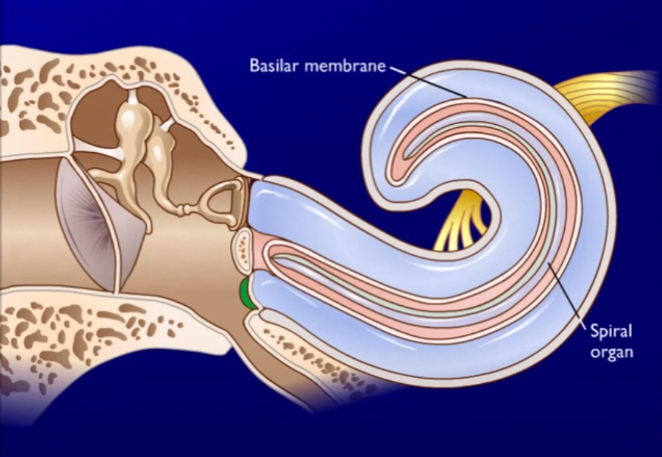
\includegraphics[width=\textwidth]{basilar}
\end{figure}
\begin{itemize}
    \item{In Cochlea, specifically organ of corti}
    \item{Covered in hair cells}
    \item{Converts waves of fluid into electrical impulses}
    \item{Oval window vibrates fluid of cochlea, \hl{producing waves that bend the hairs} of basilar membrane, producing an electrical impulse}
\end{itemize}

\begin{figure}[H]
    \centering
    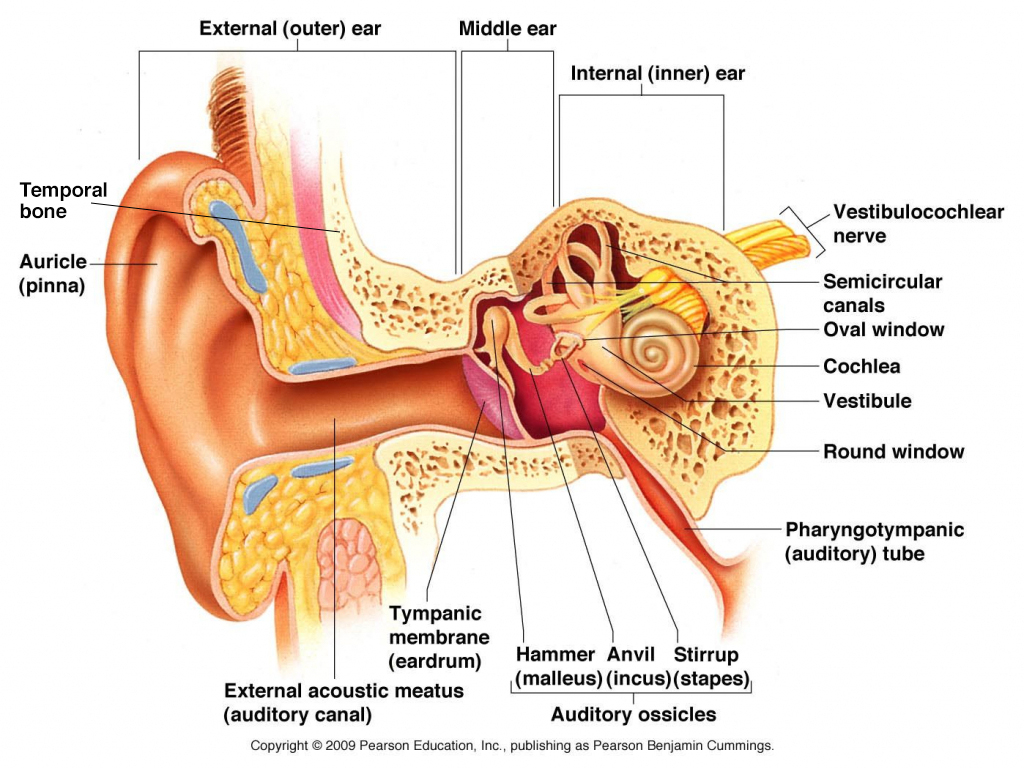
\includegraphics[width=\textwidth]{ear2}
\end{figure}

\section{Hearing Loss}
\subsection{Intense Sound Response}
\begin{itemize}
    \item{Muscles contract, restricting movement of malleus of ossicles}
    \item{Second muscle contracts, pulling stapes away from oval window}
\end{itemize}

\subsection{Types}
\begin{itemize}
    \item{\textbf{Conductive hearing loss}\\= caused by wax build-up, middle ear infection, or punctured eardrum}
    \item{
            \textbf{Sensorineural hearing loss}\\= auditory nerve severed, or cochlea hair cells damaged
            \begin{itemize}
                \item{caused by aging, loud noises, head trauma, or genetic conditions}
            \end{itemize}
        }
\end{itemize}

\subsection{Treatments}
\begin{itemize}
    \item{\textbf{Hearing aid} = amplfies sound, auditory nerve intact}
    \item{\textbf{Cochlear implant} = auditory nerve bypass}
\end{itemize}

\subsection{Tinnitus}
\begin{itemize}
    \item{Ringing in ear}
    \item{Malfunction of cochlea --- hair cells are damaged, bent, or destroyed}
    \item{Loss of hair cells as we age}
\end{itemize}

\section{Balance and Equilibrium}
\subsection{Rotational/Dynamic Equilibrium}
\begin{itemize}
    \item{Balance is maintained by the three fluid filled semicircular canals}
    \item{\textbf{Ampulla} = pocket containing hair cells filled cupula}
    \item{\textbf{Cupula} = gel-like substance that is moved by gravity or centrifugal force}
    \item{The \hl{movement of the gel} \hl{bends the cilia} hair cells, initiating nerve impulses}
\end{itemize}

\subsection{Gravitational/Static Equilibrium}
\begin{itemize}
    \item{Detects head position}
    \item{
            Maintained by two fluid filled sacs which make up \textbf{vestibule}
            \begin{itemize}
                \item{\textbf{Saccule}}
                \item{\textbf{Utricle}}
            \end{itemize}
        }
    \item{Each sac contains hair-like receptors suspended in a jelly-like substance}
    \item{\textbf{Otoliths} = each sac contains these tiny stones, which help move the jelly-like substance}
\end{itemize}

\end{document}
